% Copyright (c) 2012 Raniere Silva <r.gaia.cs@gmail.com>
% Copyright (c) 2012 Fernando Cezarino <feolce@gmail.com>
% Copyright (c) 2012 Ana Paula Diniz Marques <anapdinizm@gmail.com>
% Copyright (c) 2012 Camile Kunz <camileknz@gmail.com>
% Copyright (c) 2012 Ana Flavia <anaflavia.c.lima@gmail.com>
%
% This file is part of 'MS480 - 2012S2 - Aterro com Obstáculo'.
%
% 'MS480 - 2012S2 - Aterro com Obstáculo' is licensed under the Creative Commons
% Attribution-ShareAlike 3.0 Unported License. To view a copy of this license,
% visit http://creativecommons.org/licenses/by-sa/3.0/.
%
% 'MS480 - 2012S2 - Aterro com Obstáculo' is distributed in the hope that it
% will be useful, but WITHOUT ANY WARRANTY; without even the implied warranty of
% MERCHANTABILITY or FITNESS FOR A PARTICULAR PURPOSE.
\section{Modelagem}
A seguir apresentamos a modelagem proposta por Andjel e depois expandimos essa
modelagem para o problema a ser tratado. Ao final, abordamos a questão da
distância.

\subsection{Problema sem obstáculo}
Considere a Figura~\ref{fig:ilust_J_A} em que é representado as regiões $A$ e
$J$.
\begin{figure}[!htb]
    \centering
    \begin{tikzpicture}
        \draw[pattern=bricks](0,0) rectangle (2,2) node[fill=white,
        midway]{$A$};
        \draw[pattern=checkerboard] (6,6) rectangle (8,8) node[fill=white,
        midway]{$J$};

        % Escala
        \node[fill=white, above] at (5,1.2) {$0$};
        \draw[fill=black] (5,1) rectangle (6,1.2) node[fill=white, above]{$e$};
        \draw[fill=white] (6,1) rectangle (7,1.2) node[fill=white, above]{$2e$};
        \draw[fill=black] (7,1) rectangle (8,1.2) node[fill=white, above]{$3e$};
    \end{tikzpicture}
    \caption{Ilustra\c{c}\~{a}o das regiões $J$ e $A$.}
    \label{fig:ilust_J_A}
\end{figure}

Para modelarmos o problema, discretizamos a região ilustrada na
Figura~\ref{fig:ilust_J_A} utilizando uma malha quadriculada como, ilustrado na
Figura~\ref{fig:disc_J_A}, e nomeamos cada quadrado da malha por um número
seguindo a lógica indicada na Figura~\ref{fig:disc_J_A}.
\begin{figure}[!htb]
    \centering
    \begin{tikzpicture}
        \draw[color=gray, step=.5] (0,0) grid (8,8);
        \draw[->] (-.2,8) -- (8.2,8);
        \draw[->] (0,-.2) -- (0,8.2);

        \draw[pattern=bricks](0,0) rectangle (2,2) node[fill=white,
        midway]{$A$};
        \draw[pattern=checkerboard] (6,6) rectangle (8,8) node[fill=white,
        midway]{$J$};

        \foreach \x in {1,...,12}{
            \node at (\x/2 - .25,7.75) {\small{$\x$}};
        }
        \foreach \x in {17,...,28}{
            \node at (\x/2 - 8.25,7.25) {\small{$\x$}};
        }

        % Escala
        \node[fill=white, above] at (5,1.2) {$0$};
        \draw[fill=black] (5,1) rectangle (6,1.2) node[fill=white, above]{$e$};
        \draw[fill=white] (6,1) rectangle (7,1.2) node[fill=white, above]{$2e$};
        \draw[fill=black] (7,1) rectangle (8,1.2) node[fill=white, above]{$3e$};
    \end{tikzpicture}
    \caption{Ilustra\c{c}\~{a}o das regiões $J$ e $A$.}
    \label{fig:disc_J_A}
\end{figure}

Seja $\phi : J \to \mathbb{R}$, $\psi: A \to \mathbb{R}$, $f: (J, A) \to
\mathbb{R}$ e $d: (J, A) \to \mathbb{R}$, onde $\phi(x)$ corresponde ao volume
de terra disponível no quadrado $x$, $\psi(y)$ ao volume de terra necessário no
quadrado $y$, $f(x,y)$ ao volume de terra transportado do quadrado $x$ para o
quadrado $y$ e $d(x, y)$ a distância entre os quadrados $x$ e $y$.

Sendo $\xi_{x,y}$ a variável de decisão correspondente ao volume de terra
transportado de $x$ para $y$, podemos modelar o problema da seguinte forma:
\begin{subequations}
    \begin{align}
        \text{max } & \sum_{x \in J} \sum_{y \in A} \xi_{x,y},
        \label{eq:model_without_obs:obj_func} \\
        \text{s.a. } & \xi_{x,y} \geq 0, && \forall x, y \in N,
        \label{eq:model_without_obs:var} \\
        & \xi_{x,y} = 0 && \forall d(x,y) > D,
        \label{eq:model_without_obs:max_dist} \\
        & \sum_{y \in A} \xi_{x,y} \leq \phi(x), && \forall x \in J,
        \label{eq:model_without_obs:max_jazida} \\
        & \sum_{x \in J} \xi_{x,y} \leq \psi(y), && \forall y \in A,
        \label{eq:model_without_obs:max_aterro}
    \end{align}
    \label{eq:model_without_obs}
\end{subequations}
onde \eqref{eq:model_without_obs:max_dist} refere-se a distância máxima dos
canos utilizados, \eqref{eq:model_without_obs:max_jazida} a quantidade de terra
que pode ser retirado de $J$ e \eqref{eq:model_without_obs:max_aterro} a
quantidade de terra necessário e $A$.

\subsection{Problema com obstáculo}
Trataremos o problema descrito em sua forma discreta, i.e., dado um valor
$\delta$ definimos uma malha quadriculada que cobre toda a regi\~{a}o de
interesse como na Figura~\ref{fig:malha_quad}. Cada elemento da malha
quadriculada recebe uma identificação numérica como ilustrada na
Figura~\ref{fig:malha_quad_num}.
\begin{figure}[!htb]
    \centering
    \begin{tikzpicture}
        \draw[color=gray] (0,0) grid (8,8);
        \draw[->] (-.2,8) -- (8.2,8);
        \draw[->] (0,-.2) -- (0,8.2);

        \draw[pattern=bricks](0,0) rectangle (2,2) node[fill=white,
        midway]{$A$};
        \draw[pattern=fivepointed stars] (4,4) node[fill=white]{$R$}
        circle (1.7) ;
        \draw[pattern=checkerboard] (6,6) rectangle (8,8) node[fill=white,
        midway]{$J$};

        \draw[<->] (6,1) -- (7,1) node[midway, below]{$\delta$};
    \end{tikzpicture}
    \caption{Ilustra\c{c}\~{a}o da malha quadricular sobre a regi\~{a}o de
    interesse.}
    \label{fig:malha_quad}
\end{figure}
\begin{figure}[!htb]
    \centering
    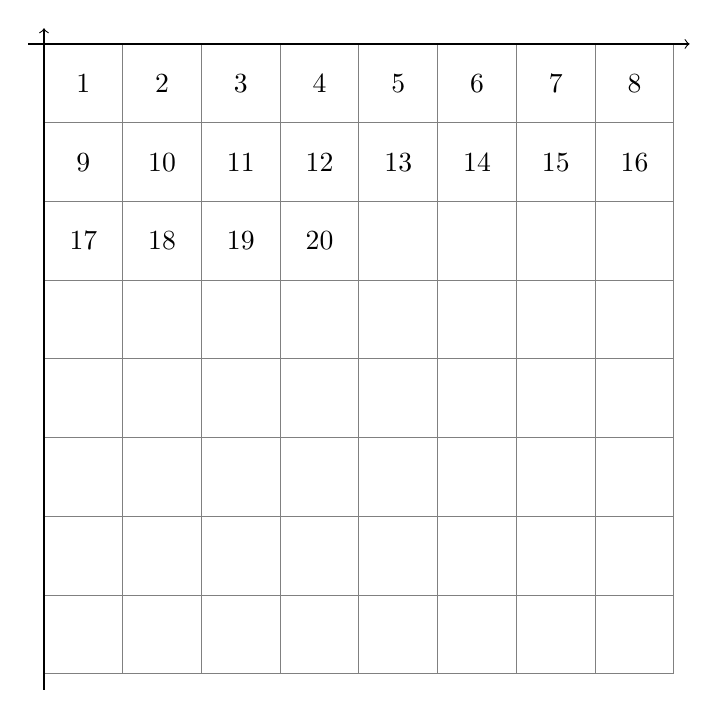
\begin{tikzpicture}
        \draw[color=gray] (0,0) grid (8,8);
        \draw[->] (-.2,8) -- (8.2,8);
        \draw[->] (0,-.2) -- (0,8.2);

        \foreach \x in {1,...,8}{
            \node at (\x - .5,7.5) {$\x$};
        }
        \foreach \x in {9,...,16}{
            \node at (\x - 8.5,6.5) {$\x$};
        }
        \foreach \x in {17,...,20}{
            \node at (\x - 16.5,5.5) {$\x$};
        }
    \end{tikzpicture}
    \caption{Ilustra\c{c}\~{a}o da numeração da malha quadricular.}
    \label{fig:malha_quad_num}
\end{figure}

Seja $\phi : J \to \mathbb{R}$, $\psi: A \to \mathbb{R}$ e $f: (J, A) \to \mathbb{R}$,
onde $\phi(x)$ corresponde ao volume de terra disponível na célula $x$, $\psi(y)$
ao volume de terra necessário na célula $y$, $f(x,y)$ ao volume de terra
transportado da célula $x$ para a célula $y$ e $d(x, y)$ a distância entre as
células $x$ e $y$\footnote{A distância entre as células $x$ e $y$ será definida
posteriormente.}. Seja também $D$ o comprimento dos canos disponíveis, $J$ o
conjunto de células que compõem a jazida e $A$ o conjunto de células que compõem
o aterro.

Então, podemos modelar o problema da seguinte forma
\begin{subequations}
    \begin{align}
        \text{min } & \sum_{x \in J} \sum_{y \in A} \xi_{x,y},
        \label{eq:model_with_obs:obj_func} \\
        \text{s.a. } & \xi_{x,y} \geq 0, && \forall x, y \in N,
        \label{eq:model_with_obs:var} \\
        & \xi_{x,y} = 0 && \forall d_{x,y} > D,
        \label{eq:model_with_obs:max_dist} \\
        & \sum_{y \in A} \xi_{x,y} \leq \phi(x), && \forall x \in J,
        \label{eq:model_with_obs:max_jazida} \\
        & \sum_{x \in J} \xi_{x,y} \leq \psi(y), && \forall y \in A,
        \label{eq:model_with_obs:max_aterro}
    \end{align}
    \label{eq:model_with_obs}
\end{subequations}

\subsection{Distância entre pontos}
Ao utilizar a malha quadriculada podemos definir a dist\^{a}ncia entre dois
quadrados da malha de pelo menos tr\^{e}s maneiras diferentes:
\begin{enumerate}
    \item $d_l$, que \'{e} a menor dist\^{a}ncia entre qualquer dois pontos dos
        quadrados,
    \item $d_u$, que \'{e} a maior dist\^{a}ncia entre qualquer dois pontos dos
        quadrados, e
    \item $d_c$, que \'{e} a dist\^{a}ncia entre os centros dos quadrados.
\end{enumerate}
Na Figura~\ref{fig:dist_malha} \'{e} ilustrado cada uma das dist\^{a}ncias acima
descrita.
\begin{figure}[!htb]
    \centering
    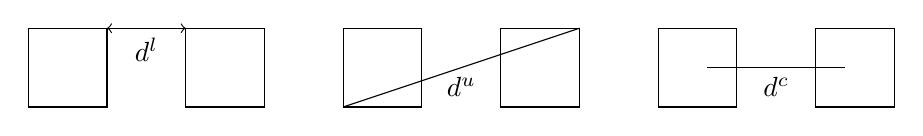
\begin{tikzpicture}
        \draw (0,0) rectangle (1,1);
        \draw (2,0) rectangle (3,1);
        \draw[<->] (1,1) -- (2,1) node[midway, below]{$d^l$};

        \draw (4,0) rectangle (5,1);
        \draw (6,0) rectangle (7,1);
        \draw (4,0) -- (7,1) node[midway, below]{$d^u$};

        \draw (8,0) rectangle (9,1) node[midway](A){};
        \draw (10,0) rectangle (11,1) node[midway](B){};
        \draw (A) -- (B) node[midway, below]{$d^c$};
    \end{tikzpicture}
    \caption{Ilustra\c{c}\~{a}o das dist\^{a}ncias entre quadrados da malha.}
    \label{fig:dist_malha}
\end{figure}

Quanto ao obst\'{a}culo
